\documentclass[class=minimal]{standalone}

\usepackage{tikz}

\begin{document}

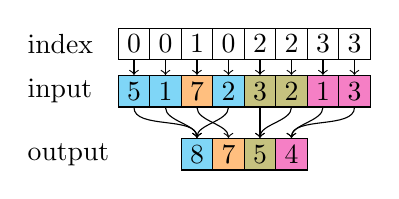
\begin{tikzpicture}

\tikzstyle{title}=[text width=1.1cm, inner sep=0pt]
\tikzstyle{square}=[rectangle, draw, minimum width=0.4cm, minimum height=0.4cm, inner sep=0pt, fill opacity=0.5, text opacity=1]
\tikzstyle{color1}=[fill=cyan]
\tikzstyle{color2}=[fill=orange]
\tikzstyle{color3}=[fill=olive]
\tikzstyle{color4}=[fill=magenta]
\tikzstyle{edge1}=[->]
\tikzstyle{edge2}=[out=-90, in=90, looseness=0.8]

\node[title] at (-0.8, 1.4) {index};
\node[title] at (-0.8, 0.8) {input};
\node[title] at (-0.8, 0.0) {output};

\node[square] (index1) at (0.0, 1.4) {$0$};
\node[square] (index2) at (0.4, 1.4) {$0$};
\node[square] (index3) at (0.8, 1.4) {$1$};
\node[square] (index4) at (1.2, 1.4) {$0$};
\node[square] (index5) at (1.6, 1.4) {$2$};
\node[square] (index6) at (2.0, 1.4) {$2$};
\node[square] (index7) at (2.4, 1.4) {$3$};
\node[square] (index8) at (2.8, 1.4) {$3$};

\node[square, color1] (input1)  at (0.0, 0.8) {$5$};
\node[square, color1] (input2)  at (0.4, 0.8) {$1$};
\node[square, color2] (input3)  at (0.8, 0.8) {$7$};
\node[square, color1] (input4)  at (1.2, 0.8) {$2$};
\node[square, color3] (input5)  at (1.6, 0.8) {$3$};
\node[square, color3] (input6)  at (2.0, 0.8) {$2$};
\node[square, color4] (input7)  at (2.4, 0.8) {$1$};
\node[square, color4] (input8)  at (2.8, 0.8) {$3$};

\node[square, color1] (output1)  at (0.8, 0.0) {$8$};
\node[square, color2] (output2)  at (1.2, 0.0) {$7$};
\node[square, color3] (output3)  at (1.6, 0.0) {$5$};
\node[square, color4] (output4)  at (2.0, 0.0) {$4$};

\draw[edge1] (index1) -- (input1);
\draw[edge1] (index2) -- (input2);
\draw[edge1] (index3) -- (input3);
\draw[edge1] (index4) -- (input4);
\draw[edge1] (index5) -- (input5);
\draw[edge1] (index6) -- (input6);
\draw[edge1] (index7) -- (input7);
\draw[edge1] (index8) -- (input8);

\draw[edge1] (input1) to[edge2] (output1);
\draw[edge1] (input2) to[edge2] (output1);
\draw[edge1] (input3) to[edge2] (output2);
\draw[edge1] (input4) to[edge2] (output1);
\draw[edge1] (input5) to[edge2] (output3);
\draw[edge1] (input6) to[edge2] (output3);
\draw[edge1] (input7) to[edge2] (output4);
\draw[edge1] (input8) to[edge2] (output4);

\end{tikzpicture}

\end{document}
